% A LaTeX template for MSc Thesis submissions to 
% Politecnico di Milano (PoliMi) - School of Industrial and Information Engineering
%
% S. Bonetti, A. Gruttadauria, G. Mescolini, A. Zingaro
% e-mail: template-tesi-ingind@polimi.it
%
% Last Revision: October 2021
%
% Copyright 2021 Politecnico di Milano, Italy. NC-BY

\documentclass{Configuration_Files/PoliMi3i_thesis}

%------------------------------------------------------------------------------
%	REQUIRED PACKAGES AND  CONFIGURATIONS
%------------------------------------------------------------------------------

% CONFIGURATIONS
\usepackage{parskip} % For paragraph layout
\usepackage{setspace} % For using single or double spacing
\usepackage{emptypage} % To insert empty pages
\usepackage{multicol} % To write in multiple columns (executive summary)
\setlength\columnsep{15pt} % Column separation in executive summary
\setlength\parindent{0pt} % Indentation
\raggedbottom  

% PACKAGES FOR TITLES
\usepackage{titlesec}
% \titlespacing{\section}{left spacing}{before spacing}{after spacing}
\titlespacing{\section}{0pt}{3.3ex}{2ex}
\titlespacing{\subsection}{0pt}{3.3ex}{1.65ex}
\titlespacing{\subsubsection}{0pt}{3.3ex}{1ex}
\usepackage{color}

% PACKAGES FOR LANGUAGE AND FONT
\usepackage[english]{babel} % The document is in English  
\usepackage[utf8]{inputenc} % UTF8 encoding
\usepackage[T1]{fontenc} % Font encoding
\usepackage[11pt]{moresize} % Big fonts

% PACKAGES FOR IMAGES
\usepackage{graphicx}
\usepackage{transparent} % Enables transparent images
\usepackage{eso-pic} % For the background picture on the title page
\usepackage{subfig} % Numbered and caption subfigures using \subfloat.
\usepackage{tikz} % A package for high-quality hand-made figures.
\usetikzlibrary{}
\graphicspath{{./Images/}} % Directory of the images
\usepackage{caption} % Coloured captions
\usepackage{xcolor} % Coloured captions
\usepackage{amsthm,thmtools,xcolor} % Coloured "Theorem"
\usepackage{float}

% STANDARD MATH PACKAGES
\usepackage{amsmath}
\usepackage{amsthm}
\usepackage{amssymb}
\usepackage{amsfonts}
\usepackage{bm}
\usepackage[overload]{empheq} % For braced-style systems of equations.
\usepackage{fix-cm} % To override original LaTeX restrictions on sizes

% PACKAGES FOR TABLES
\usepackage{tabularx}
\usepackage{longtable} % Tables that can span several pages
\usepackage{colortbl}

% PACKAGES FOR ALGORITHMS (PSEUDO-CODE)
\usepackage{algorithm}
\usepackage{algorithmic}

% PACKAGES FOR REFERENCES & BIBLIOGRAPHY
\usepackage[colorlinks=true,linkcolor=black,anchorcolor=black,citecolor=black,filecolor=black,menucolor=black,runcolor=black,urlcolor=black]{hyperref} % Adds clickable links at references
\usepackage{cleveref}
\usepackage[square, numbers, sort&compress]{natbib} % Square brackets, citing references with numbers, citations sorted by appearance in the text and compressed
\bibliographystyle{abbrvnat} % You may use a different style adapted to your field

% OTHER PACKAGES
\usepackage{pdfpages} % To include a pdf file
\usepackage{afterpage}
\usepackage{lipsum} % DUMMY PACKAGE
\usepackage{fancyhdr} % For the headers
\fancyhf{}

% Input of configuration file. Do not change config.tex file unless you really know what you are doing. 
% Define blue color typical of polimi
\definecolor{bluepoli}{cmyk}{0.4,0.1,0,0.4}

% Custom theorem environments
\declaretheoremstyle[
  headfont=\color{bluepoli}\normalfont\bfseries,
  bodyfont=\color{black}\normalfont\itshape,
]{colored}

% Set-up caption colors
\captionsetup[figure]{labelfont={color=bluepoli}} % Set colour of the captions
\captionsetup[table]{labelfont={color=bluepoli}} % Set colour of the captions
\captionsetup[algorithm]{labelfont={color=bluepoli}} % Set colour of the captions

\theoremstyle{colored}
\newtheorem{theorem}{Theorem}[chapter]
\newtheorem{proposition}{Proposition}[chapter]

% Enhances the features of the standard "table" and "tabular" environments.
\newcommand\T{\rule{0pt}{2.6ex}}
\newcommand\B{\rule[-1.2ex]{0pt}{0pt}}

% Pseudo-code algorithm descriptions.
\newcounter{algsubstate}
\renewcommand{\thealgsubstate}{\alph{algsubstate}}
\newenvironment{algsubstates}
  {\setcounter{algsubstate}{0}%
   \renewcommand{\STATE}{%
     \stepcounter{algsubstate}%
     \Statex {\small\thealgsubstate:}\space}}
  {}

% New font size
\newcommand\numfontsize{\@setfontsize\Huge{200}{60}}

% Title format: chapter
\titleformat{\chapter}[hang]{
\fontsize{50}{20}\selectfont\bfseries\filright}{\textcolor{bluepoli} \thechapter\hsp\hspace{2mm}\textcolor{bluepoli}{|   }\hsp}{0pt}{\huge\bfseries \textcolor{bluepoli}
}

% Title format: section
\titleformat{\section}
{\color{bluepoli}\normalfont\Large\bfseries}
{\color{bluepoli}\thesection.}{1em}{}

% Title format: subsection
\titleformat{\subsection}
{\color{bluepoli}\normalfont\large\bfseries}
{\color{bluepoli}\thesubsection.}{1em}{}

% Title format: subsubsection
\titleformat{\subsubsection}
{\color{bluepoli}\normalfont\large\bfseries}
{\color{bluepoli}\thesubsubsection.}{1em}{}

% Shortening for setting no horizontal-spacing
\newcommand{\hsp}{\hspace{0pt}}

\makeatletter
% Renewcommand: cleardoublepage including the background pic
\renewcommand*\cleardoublepage{%
  \clearpage\if@twoside\ifodd\c@page\else
  \null
  \AddToShipoutPicture*{\BackgroundPic}
  \thispagestyle{empty}%
  \newpage
  \if@twocolumn\hbox{}\newpage\fi\fi\fi}
\makeatother

%For correctly numbering algorithms
\numberwithin{algorithm}{chapter}

%----------------------------------------------------------------------------
%	NEW COMMANDS DEFINED
%----------------------------------------------------------------------------


%----------------------------------------------------------------------------
%	ADD YOUR PACKAGES (be careful of package interaction)
%----------------------------------------------------------------------------

\usepackage[innercaption]{sidecap}
\usepackage{wrapfig}

%----------------------------------------------------------------------------
%	ADD YOUR DEFINITIONS AND COMMANDS (be careful of existing commands)
%----------------------------------------------------------------------------

\newcommand{\easyfly}{EasyFly}
\newcommand{\HRI}{Human-Robot Interactions}
\newcommand{\hri}{Human-Robot interactions}
\newcommand{\HDI}{Human-Drone Interactions}
\newcommand{\hdi}{Human-Drone interactions}
\newcommand{\Dronearena}{Drone Arena Challenge}

%----------------------------------------------------------------------------
%	BEGIN OF YOUR DOCUMENT
%----------------------------------------------------------------------------

\begin{document}

\fancypagestyle{plain}{%
\fancyhf{} % Clear all header and footer fields
\fancyhead[RO,RE]{\thepage} %RO=right odd, RE=right even
\renewcommand{\headrulewidth}{0pt}
\renewcommand{\footrulewidth}{0pt}}

%----------------------------------------------------------------------------
%	TITLE PAGE
%----------------------------------------------------------------------------

\pagestyle{empty} % No page numbers
\frontmatter % Use roman page numbering style (i, ii, iii, iv...) for the preamble pages

\puttitle{
	title=Programming Environment for \\Human Drone Interaction: EasyFly, % Title of the thesis
	name=Matteo Plona, % Author Name and Surname
	course=Computer Science Engineering, % Study Programme (in Italian)
	ID  = 952967,  % Student ID number (numero di matricola)
	advisor= Prof. Luca Mottola, % Supervisor name
	%coadvisor={Name Surname}, % Co-Supervisor name, remove this line if there is none
	academicyear={2023-24},  % Academic Year
} % These info will be put into your Title page 

%----------------------------------------------------------------------------
%	PREAMBLE PAGES: ABSTRACT (inglese e italiano), EXECUTIVE SUMMARY
%----------------------------------------------------------------------------
\startpreamble
\setcounter{page}{1} % Set page counter to 1

% ABSTRACT IN ENGLISH
\chapter*{Abstract} 
TODO



%Here goes the Abstract in English of your thesis followed by a list of keywords.
%The Abstract is a concise summary of the content of the thesis (single page of text)
%and a guide to the most important contributions included in your thesis.
%The Abstract is the very last thing you write.
%It should be a self-contained text and should be clear to someone who hasn't (yet) read the whole manuscript.
%The Abstract should contain the answers to the main scientific questions that have been addressed in your thesis.
%It needs to summarize the adopted motivations and the adopted methodological approach as well as the findings of your work and their relevance and impact.
%The Abstract is the part appearing in the record of your thesis inside POLITesi,
%the Digital Archive of PhD and Master Theses (Laurea Magistrale) of Politecnico di Milano.
%The Abstract will be followed by a list of four to six keywords.
%Keywords are a tool to help indexers and search engines to find relevant documents.
%To be relevant and effective, keywords must be chosen carefully.
%They should represent the content of your work and be specific to your field or sub-field.
%Keywords may be a single word or two to four words.
\textbf{Keywords:} here, the keywords, of your thesis % Keywords

% ABSTRACT IN ITALIAN
\chapter*{Abstract in lingua italiana}
TODO



%Qui va l'Abstract in lingua italiana della tesi seguito dalla lista di parole chiave.
\textbf{Parole chiave:} qui, vanno, le parole chiave, della tesi % Keywords (italian)

%----------------------------------------------------------------------------
%	LIST OF CONTENTS/FIGURES/TABLES/SYMBOLS
%----------------------------------------------------------------------------

% TABLE OF CONTENTS
\thispagestyle{empty}
\tableofcontents % Table of contents 
\thispagestyle{empty}
\cleardoublepage

%-------------------------------------------------------------------------
%	THESIS MAIN TEXT
%-------------------------------------------------------------------------

\addtocontents{toc}{\vspace{2em}} % Add a gap in the Contents, for aesthetics
\mainmatter % Begin numeric (1,2,3...) page numbering

% --------------------------------------------------------------------------
% CHAPTERS 
% --------------------------------------------------------------------------
\chapter{Introduction}
\label{ch:intro}
In recent years, the rapid advancement of unmanned aerial vehicles, commonly known as drones,
has revolutionized various industries and opened up new possibilities for applications ranging
from aerial photography and package delivery to search and rescue operations. As drones become
increasingly integrated into our daily lives, it is crucial to explore and understand the dynamics
of their interaction with humans.

In modern drone applications, the human figure is marginal with respect to the drone.
The former usually plays the supervisor role, where the main task is to control the activities and check that every operation is carried out correctly. 
At the same time, the latter performs almost all requested tasks automatically.
This significant discrepancy undoubtedly leads to a decrease in interactions between the two.

This thesis will describe EasyFly, an accessible and high-level programming environment for drone applications.
The purpose is to provide a programming environment to allow users with different levels of expertise to experiment with drones. 
Differently from modern applications, our environment allows humans and drones to work closely together,
making EasyFly a perfect tool for conducting research in the field of human-drone interactions.


\section{The Problem: Programming Human-Drone Interactions}\label{sec:the_problem}
Human-Drone Interaction (HDI) is a branch of the more general field of Human-Robot Interaction (HRI), and it can be defined as 
`the study field focused on understanding, designing, and evaluating drone systems for use by or with human user~\cite{tezza2019hdi}`.
While the field of HRI offers valuable insights, the distinctive ability of drones to move freely in three-dimensional
space, along with their unique shapes, sets HDI as a distinct and independent area of research.

The rapid technological progress in this field has made drones increasingly efficient and autonomous in performing various
tasks. While on the one hand, these advancements enable the integration of drones into everyday life, streamlining processes
and reducing the time required for specific activities, on the other hand, modern drone applications do not represent the
ideal prototype for conducting research in the field of HDI.

The first limitation of modern drone applications in this discipline's study is that these applications are designed
to operate in large environments with minimal human presence. An example can be represented by autonomous delivery
drones~\cite{singireddy2018primeAir} or 3D mapping applications~\cite{nex3Dmapping} where the interactions with the human are purposely
reduced to the bare minimum.

In these types of applications, interactions between humans and drones are often limited to simple tasks, such as package
delivery or crop monitoring. These interactions are often repetitive and lack the diversity and complexity required in
research on HDI. Since tasks and interactions are repetitive, users are usually trained to interact with the drone
in a specific way. This training can reduce the variability in HDI, making it less suitable for research purposes.

Programming HDI is usually the field's most complex and expensive task. 
Usually, researchers in this field are unfamiliar with programming at low-level embedded systems like drones.
For this reason, a specialized team of researchers is typically required to program a custom drone application that addresses the complexity of the interactions requested. 

Moreover, the implementation phase is usually the bottleneck of the entire process; every small change to the interaction model can result in days or weeks for implementing the desired behavior.
In fact, one of the most significant challenges during the programming of HDI is the testing phase.
Modern drones are usually fragile and expensive, while tests are likely to fail. 
This phase usually introduces a high consumption of resources, both in terms of costs and time needed for repairing the entire setup before another attempt.


\section{The Solution: EasyFly}\label{sec:the_solution}
To overcome the issues related to the programming of HDI, we introduce EasyFly, a programming environment for drone applications that addresses all the research needs in the field of HDI.

To better understand the contribution of EasyFly to this research field, let us take a step back and describe the needs of researchers.

The ideal prototype of a programming environment for researchers studying HDI should address and solve all the problems related to developing drone applications used for research. 
In particular, this prototype should ultimately reduce the time and costs associated with the development phase and increase the research's effectiveness.

The first characteristic of the ideal prototype is to reduce the level of expertise needed to develop the desired drone application. 
This feature allows researchers to easily implement all the required functionality without requiring a specialized drone programmer team. 
Moreover, this feature would open the doors to a brand-new type of research where the users interact with the drone programmed by themselves.
EasyFly provides this feature by offering a set of simple operations, which indeed allows the creation of very complex behaviors.
In addition to this, EasyFly allows programming in a descriptive fashion; in this way, programs would be self-explaining and easily interpreted by anyone.

As in any other field, research on HDI should be dynamic. 
In other words, to gather all the possible insights from an interaction, the drone application must rapidly change and adapt to the situation.
If the application development cycle is too long, there is the risk of losing many possible opportunities to experiment with possible alternative solutions. 
The ideal prototype should provide the maximum flexibility in adapting to many possible situations.
For this reason, EasyFly has adopted a modular approach for both the hardware and the software components.
At any moment, a module (either software or hardware) can be attached or detached to compose the best configuration needed at that specific moment.

Last but not least, facilitating the interaction between the human and the drone should be the primary goal.
The ideal prototype should be the first promoter of the interaction. 
It should offer the best possible condition to allow the two entities to establish an interaction safely and free from any potential bias determined by the programming environment.
In other words, it should use a typology of drones that allow close contact.

To implement EasyFly, we have targeted a specific typology of unmanned aerial vehicles: nano-drones.
As the name suggests, nano-drones are simply drones with very small size and weight. Their small size makes them the best choice to facilitate human-drone interaction.

In the first place, nano-drones are less intimidating and intrusive than larger drones, making it easier for
researchers to observe how individuals react and interact with them. They also allow minimal disturbance in the
observation environment, making them perfect for avoiding any possible noise in the experiment.
Given that the drone and the human are supposed to work closely together, any possible malfunction can cause an unexpected drone crash, 
especially while experimenting with new solutions. It is easy to deduce that the smaller the drone is, the safer the interaction.
The last observation is that nano-drones are usually less expensive than bigger ones, allowing researchers
to experiment with interactions with multiple drones without affecting their budget.


\section{The Benchmark: Drone Arena Challenge}\label{sec:the_benchmark}
In the HDI domain, the research's core part, especially from the computer science perspective,
is the experimental phase. During this phase, researchers put their ideas and prototypes to test
and assess the practicality of innovative interaction models.

For a programming environment like EasyFly, testing and evaluating in a real research scenario in HDI is essential. 
The testing in real scenarios can help detect possible weaknesses in the programming environment, allowing for fine-tuning the model.

To best evaluate our EasyFly programming environment, we had the possibility to participate in the Digital Futures Drone Arena project~\cite{dronearena}.
This project allowed us to perform an in-depth analysis of the impact of using EasyFly while developing human-drone interactions. 

Drone Arena is an interdisciplinary research project that aims to create a technological and conceptual platform for interdisciplinary investigations of drones at the intersection of mobile robotics,
 autonomous systems, machine learning, and Human-Computer Interaction.
The project has three inter-related objectives:
\begin{enumerate}
    \item   The constructions of a novel aerial drone testbed that is geared towards application-level
            functionality rather than low-level control mechanisms.
    \item   The organization of two challenges where multiple teams are involved and tasked to realize
            functionality that pushes the state of the art.
    \item   Conducting empirical investigation of Human Drone Interactions in the Drone Arena.
            This includes observation, interviews, and micro-sociological video analysis to inform future
            competitions in the drone arena and to develop insights from the movement-based explorations of drone piloting.
\end{enumerate}

In these settings, our EasyFly programming environment is focused on the first two objectives.
In particular, our programming environment was one of the core parts of the novel aerial drone testbed used for the entire duration of the project. 
For the second objective of the project, we had the possibility to actively participate in the first of the two challenges organized for the Drone Arena project. 
During this challenge, we conducted a complete and in-depth evaluation of the impact of using EasyFly; 
in particular, we compared our programming environment with a simpler and lower-level one.


\section{State of the Art}\label{sec:intro_soa}
The field of HDI is an active and evolving area of research with a focus on improving the ways in which humans
and drones interact. It is a multidisciplinary field with two main research areas: technological and sociological.
Each area focuses on distinct aspects of the interaction between humans and drones~\cite{hri2009davidMaya}.

In the technological area, at the intersection of computer science, mobile robotics, autonomous systems, and machine learning,
the key focus is developing and improving the hardware and software components of drones and their interfaces~\cite{kolling2012towards, giusti2012distributed}.
The main goal of this area is to enhance the capabilities and functionality of drones to make them more user-friendly and efficient~\cite{cauchard2015droneAndMe}.

In the sociological area, which includes disciplines like social engineering, art, ethics, and political science,
the core objective is to understand how the presence and use of drones impact society, individuals, and communities~\cite{eriksson2020ethicsInMovement, anderson2012accidentally}.

Especially in research focused on the sociological area, where researchers usually have less familiarity with programming tools, 
the prototyping phase is the most complex and time-consuming. 
EasyFly tries to overcome all the issues related to this phase by creating a simple and flexible programming environment for drone applications.
Moreover, it tries to offer a new perspective in the investigation of human-drone interactions where the user plays the role of the programmer.

\section{Overview}\label{sec:intro_overview}

TODO at the end

\chapter{State of The Art}
\label{ch:soa}
In this chapter, we will analyze the literature and background: we will first examine the more general field of Human-Computer Interaction (HCI), passing then to Human-Robot Interaction (HRI) and, finally, Human-Drone Interaction (HDI), what are the purposes, the achievement, and the limitations of this research. 
Next, we will move to the programming environments for both single and multiple drones, understanding 
which are the main design paradigms and solutions available. 


\section{Human-Robot Interaction}\label{sec:soa_hri}
We live in an era where humans and computers are increasingly in close contact. In the last 40 years, the continuous and exponential growth 
in computational power and storage capacity, but even more relevant, the huge spread of technologies in every aspect of our lives,
has moved the concept of Human-Computer interaction to a central stage of research. 
With the massive amount of new designs of technologies and systems, this relation grows exponentially in complexity, 
and the importance of profoundly understanding it is a key aspect of bringing innovation to the next step and, more importantly, 
avoiding the risk of incurring harmful and undesired situations.

Human-Computer Interaction (HCI) is a discipline concerned with the design, evaluation, and implementation of interactive computing systems for human use
and with the study of major phenomena surrounding them~\cite{sinha2010human}.
The role of this discipline is to understand in depth the relation between humans and computers, creating user interfaces and experiences that are effective, efficient, and enjoyable. 
On the other side, HCI must also understand the limits and the risks associated with those new interfaces, which should guide governments around the world to regulate 
and control the expansion of such technologies in a sane manner but avoid limiting their potentiality.

Regarding our work, it is better to narrow down the concept of HCI to a subfield of research: Human-Robot Interaction (HRI). 
Actually, HRI is not only a subfield of the more general HCI; instead, it is a multidisciplinary field with the influence of HCI, 
artificial intelligence, natural language understanding, and social science.
The primary goal of HRI is to define a general human model that could lead to principles and algorithms allowing more natural and 
effective interactions between humans and robots~\cite{hri2009davidMaya}.

\subsection{The Interaction Between Human and Robot}\label{subsec:the_interaction}
The Human is an extremely sophisticated biological system characterized by an impressive, complex, and powerful brain that is the main
coordinator and central actor in the whole human system. Given this complexity, for our purpose, we can model it using
the Model Human Processor (MPH) proposed by Card, Moran, and Newell in 1983~\cite{card1986model}. 

MPH describes the Human as composed of 3 subsystems: the perceptual, motor, and cognitive systems. 
Each of them has a processor and memory.
Input in humans occurs mainly through the senses and output through the motor controls of the effectors~\cite{dix2010human}. 
Therefore, vision, hearing, and touch are the most important senses in HRI, while fingers, voice, eyes, 
head and body position are the primary effectors.

On the other hand, the computer is a straightforward machine that processes the input data that it receives into outputs. 
The processor is the leading actor in the data transformation process: it can perform arithmetic and logic operations very fast. 
Both input and output data for the computer are encoded binary sequences.

The interaction, with or without a robot, is a process of information transfer between two (or multiple) systems. 
The outputs of one system are the inputs of the other and vice versa. 
In the interaction, it is immediately evident that the human outputs are incompatible with the robot's input. 
Also, the outputs of a robot are not easily interpretable by a human. 
This profound discrepancy between the two is the domain of study for HRI; the user outputs need to be translated from body movements and voice to binary sequences, and, on the other hand, the robot outputs need to be translated from binary data to images, text, and sounds.

Initially, with computers becoming accessible to the public fifty years ago, command-line interaction was the only option for interacting with a computer. 
Today, interfaces have evolved into sophisticated forms such as advanced GUI, touchscreens, Augmented Reality, Virtual Reality, and Haptic interfaces. 
All these new interfaces make one side easier the lives of humans, but on the other side, they have inevitably brought values 
and ethics in technology design to the forefront of public debate: questions about the goals and politics of human-designed devices, 
and whether the social interactions of those devices are good, just, or fair~\cite{shilton2018hciEthics}. 

\subsection{HRI Taxonomy}\label{subsec:hri_taxonomy}
HRI is a highly heterogeneous field, and understanding the details of interactions between humans and robots is crucial for advancing this dynamic field. 
To define and better identify the diverse range of interactions between humans and robots, 
it is important to organize and classify the interactions in a structured taxonomy~\cite{yanco2004taxonomy}.

Following this taxonomy, HRI can be classified using the following attributes:

{\bfseries \scshape Task Type}:\\*
It is a high-level description of the task to be accomplished. It sets the tone for the system's design and use. 
Moreover, it implicitly represents the robot's environment. 
For example, the task classification could be \textit{urban search and rescue}, \textit{walking aid for blind people}, or \textit{hospital delivery robot}.

{\bfseries \scshape Task Criticality}:\\*
It measures the importance of getting the task done correctly in terms of its negative effects should problems occur. 
To mitigate the subjective nature of this attribute, it can take three values: \textit{high}, \textit{medium}, and \textit{low}.
The criticality classification could be \textit{high} for the urban search and rescue, \textit{medium} for the hospital delivery robot, and \textit{low} for a jogging companion robot.

{\bfseries \scshape Robot Morphology}:\\*
It can assume three values: \textit{anthropomorphic} (having a human-like appearance), \textit{zoomorphic} (having an animal-like appearance), 
and \textit{functional} (having an appearance that is neither human-like nor animal-like but is related to the robot's function).
It is an essential measure since people react differently based on their appearance.
Examples of this classification are shown in Figure~\ref{fig:robot_morphology}

{\bfseries \scshape Interaction Roles}:\\*
When humans interact with a robot, they can act in 5 different roles: \textit{supervisor} (monitor the behavior of a robot), 
\textit{operator} (control and modify the behavior of the robot), \textit{teammate} (work in cooperation together to accomplish a task), 
\textit{mechanic/programmer} (physically change the robot's hardware or software), and \textit{bystander} 
(needs to understand the robot's behavior to be in the same space).
For example, a firefighter who uses a drone for urban search and rescue assumes the role of \textit{operator} because they need to guide it to the rescue area. 
In the hospital delivery robot, the people in the hospital have the role of \textit{bystander}; they need to understand the drone behavior since they share the same space.
\\\\ % REASON FORMAT 
{\bfseries \scshape Type of Human-Robot Physical Proximity}:\\*
When interacting with the robot, a human can act at different levels of physical proximity: \textit{none} (the robot and the human are in different places), 
\textit{avoiding} (the robot is aware and avoids the user when approaching), \textit{passing} (the robot is not aware of the user, so the user needs to pass by), 
\textit{following} (the robot is aware and follows the user when approaching), 
\textit{approaching} (the robot and the user operate close without contact), and \textit{touching} (the robot and the user operate close with contact).

{\bfseries \scshape Decision Support for the Human}:\\*
It represents the type of information that is provided to operators for decision support. 
This taxonomy category has four subcategories: 
\begin{itemize}
    \item \textit{Available sensor information}: the full list of sensors available on the robot, e.g., an urban search and rescue robot could have: \textit{sonar}, \textit{LIDAR}, \textit{camera}
    \item \textit{Sensor information provided}: the partial list of sensors useful for decision support, e.g., the robot may use its sonar and LIDAR to navigate, but only a video image is provided in the interface.
    \item \textit{Type of sensor fusion}: is specified as a list of functions that combines multiple sensors available, e.g., if sonar and LIDAR values were used to build a map that was displayed, the sensor fusion list would contain \( \{\{sonar, LIDAR\} ~\square~ map \} \).
    \item \textit{Pre-processing}: is a list of functions that preprocess the values of the sensors before displaying them in the interface, e.g., if a video stream is processed before display to highlight regions of a particular color, say red, the list would include \( \{video ~\square~ highlight red regions \} \).
\end{itemize}

{\bfseries \scshape Time and Space}:\\*
Divides Human-Robot interaction into four categories based on whether the humans and robots interact at the same time (\textit{synchronous}) or different times (\textit{asynchronous}) and while in the same place (\textit{collocated}) or different places (\textit{non-collocated}).
The urban search and rescue robot is an example of \textit{synchronous} and \textit{collocated} time and space. 
In contrast, a space rover like Curiosity~\cite{curiosity} is definitely an example of \textit{asynchronous} and \textit{non-collocated}.

{\bfseries \scshape Autonomy Level and Amount of Intervention}:\\*
The autonomy level measures the percentage of time that the robot is carrying out its task on its own; 
the amount of intervention required measures the percentage of time that a human operator must be controlling the robot.

\begin{figure}[tb]
    \centering
    \subfloat[Anthropomorphic robot\label{fig:anthropomorphic_robot}]{
        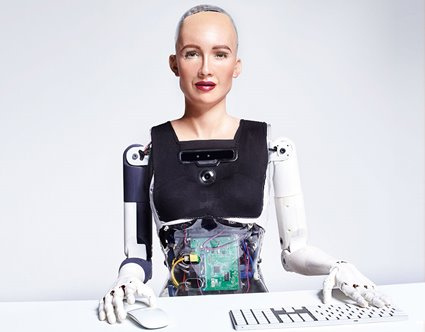
\includegraphics[width=0.28\textwidth]{soa/anthropomorphic}
    }
    \quad
    \subfloat[Zoomorphic robot\label{fig:zoomorphic_robot}]{
        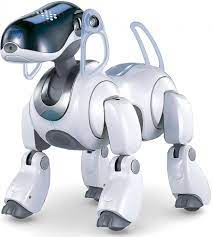
\includegraphics[width=0.28\textwidth]{soa/zoomorphic}
    }
    \quad
    \subfloat[Functional robot\label{fig:functional_robot}]{
        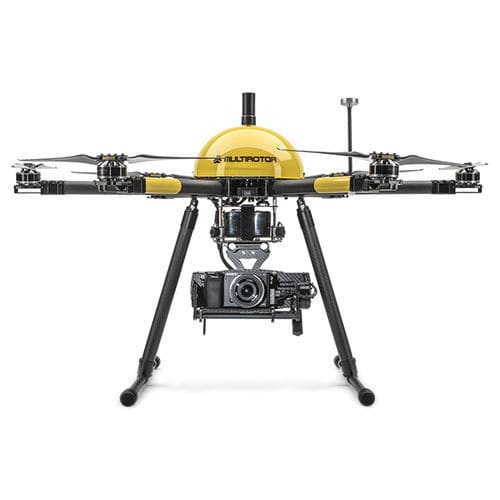
\includegraphics[width=0.28\textwidth]{soa/functional}
    }
    \caption{Robot morphology examples.}\label{fig:robot_morphology}
\end{figure}

In Table~\ref{table:taxonomy_target} we present the type of interaction that we are targeting in this thesis work using the taxonomy described above.

\begin{table}[tb]
\centering
    \begin{tabular}{|p{0.33\textwidth}|m{0.61\textwidth}|}
    \hline
    \rowcolor{bluepoli!40}
    \textbf{Attribute} & \textbf{Values} \\
    \hline \hline
    {\scshape Task Type} & Arbitrary interaction with nano drones in a small indoor environment to investigate Human-Drone relation \\
    \hline
    {\scshape Task Criticality} & Low \\
    \hline
    {\scshape Robot Morphology} & Functional \\
    \hline
    {\scshape Interaction Roles} & Mechanic/Programmer or Operator \\
    \hline
    {\scshape Physical Proximity} &  Any value \\
    \hline
    {\scshape Decision Support} & Available sensors: [proximity (x, y, z), localization (x, y, z), flow (vx, vy), video] \\
    \hline
    {\scshape Time and Space} & Synchronous and Collocated \\
    \hline
    {\scshape Autonomy Level} & Any value \\
    \hline
    {\scshape Amount of Intervention} & Any value \\
    \hline
    \end{tabular}
    \\[10pt]
    \caption[Taxonomy for interaction of target applications]{Categorization of interaction for target applications in our thesis work following the taxonomy proposed by Yanco and Drury~\cite{yanco2004taxonomy}.}\label{table:taxonomy_target}
\end{table}


\section{Human-Drone Interaction}\label{sec:soa_hdi}
Drones, also known as unmanned aerial vehicles (UAVs), are robots capable of flying autonomously or through different control modalities.
Until the early 2000s, drones were complex systems commonly seen in the military world and out of reach for civilians. 
Modern advancements in hardware and software technologies allow the development of smaller, easier-to-control, and lower-cost systems.
Drones are now found performing a broad range of civilian activities, and their usage is expected to keep increasing in the near future.
As drone usage increases, humans will interact with such systems more often; therefore, achieving a natural human-drone interaction is crucial.

Human-Drone Interaction (HDI) can be defined as the study field focused on understanding, designing, and evaluating drone systems 
for use by or with human users~\cite{tezza2019hdi}. Although some knowledge can be derived from the field of HRI, 
drones can fly in 3D space, which essentially changes how humans interact with them, making HDI a field of its own.
This field is relatively new in the research community, but in the last few years, the number of publications about HDI has grown exponentially.

\subsection{The Role of the Human During the Interaction}\label{subsec:hdi_interacction_role}
One of the core topics in the field of HDI is the role of humans during interaction with drones.
Depending on the drone's application and its level of autonomy, humans can play different roles when interacting with drone systems.

When the user pilots the drone to accomplish a given task by directly controlling the drone through a control interface, 
the user is considered an \textit{active controller} of the interaction. In these settings, the user's role is crucial to complete the given task; the drone instead acts as a mere executor of instructions. 
Examples of this type of interaction are waypoint navigation~\cite{hoppe2019droneOS} or artistic exhibitions~\cite{eriksson2020ethicsInMovement}.

The user acts as a \textit{recipient} when they do not control the drone, but they benefit from interacting with it. 
An example of this type of interaction is represented by delivery drones used to deliver a package~\cite{singireddy2018primeAir,hoppe2019droneOS, wingDrones}.

Another type of interaction role is when the drone acts as a \textit{social companion} for the user. 
In this case, the user might or might not be able to control the drone movement, but it holds a social interaction with it.
An example of this type of interaction is represented by Joggobot~\cite{graether2012joggobot}, a drone used as a companion for jogging.

The last type of role the user can play when interacting with a drone is the role of \textit{supervisor}.
Autonomous drones require users to act as supervisors either to pre-program the drone behavior or to 
supervise the flight itself in case of emergency. In this case, examples can be crop monitoring~\cite{dantu2011karma} or aerial photogrammetry~\cite{nex2014uav3Dmapping}, 

\subsection{The Drone's Control Modality}\label{subsec:hdi_drone_control_mod}
Usually, drones expose a control interface that allows users to control their behavior and eventually complete some tasks in the application domain.
Each control interface impacts how the pilot interacts with the drone in various aspects, 
such as training period, accuracy, latency, and interaction distance.

As drones became available to the public, the major drone producers felt the need to change their control modality 
from the standard remote controller to a more natural and easy-to-use interface.
A wide variety of control interfaces are available on the market today, 
ranging from standard remote controllers to very complex and advanced Brain Controlled Drones~\cite{lafleur2013quadcopterBCI}.

Drone's control interfaces can be classified as follows~\cite{tezza2019hdi}:

\textbf{\textit{Remote Controller}} is the standard and most commonly used interface, where the user directly controls the drone movements.
This control modality provides low latency and precise control, but on the other hand, it is less intuitive and usable 
than natural user interfaces. The usability and easiness of this interface strongly depend on the drone's level of autonomy.

\textbf{\textit{Gesture-based interface}} is a control modality where the user pilots the drone with body movements.
Usually, the drone uses a camera or a Kinect device to extract spatial information and recognize postures. 
When users are asked to interact with a drone without any instruction, gesture interaction is the primary choice of most users, 
and this indicates that the training period of this interface is almost close to zero~\cite{cauchard2015droneAndMe}. 
Gesture-based controls have a high latency and lower control precision compared to other control modalities. 
The flight space for drones that use this control method is sensibly reduced since the pilot needs to be close to the drone during the flight.

\textbf{\textit{Speech-based interface}} is a control modality where the user pilots the drone using vocal commands. 
As for gesture-based, this interface is also a natural user interface with a low training period and high usability.
They also share the problems of user proximity and high latency of commands.  

\textbf{\textit{Touch-based interface}} is a control modality where the user is requested to control the drone using his hands. 
The drone usually carries proximity sensors that allow it to receive inputs from the user. 
It is a natural user interface, and, like the others, it has the same pros and cons: high command latency and limited operativity distance.

\textbf{\textit{Brain-computer interfaces}} allows the user to pilot the drone using brain signals~\cite{lafleur2013quadcopterBCI}.
To enable this type of interface, the pilot must wear some form of BCI headset, the most common being 
Electroencephalography (EEG) headsets. These devices measure the brain's electrical activity on a human's scalp, 
which is decoded using machine learning algorithms to control physical systems using brain waves. 
Compared to the others, it is the most complex control interface and has the highest accessibility for users with disabilities. 
The problems in using BCI are the poor control quality and higher training period~\cite{kawala2021summary}. 
Further research in this field will probably lead to more usable and better interfaces.

Interactions can also be combined into \textbf{\textit{multimodal interfaces}}. 
Integrating different interaction methods can combine the advantages of each; however, it can increase complexity and costs.

\subsection{Values and Ethics in HDI}\label{subsec:hdi_ethics}
Drones usually carry cameras, and potentially, they can fly wherever they want; this introduces a lot of issues of privacy~\cite{anderson2012accidentally}.
Given the rapid expansion of such technology, governments worldwide have been caught off guard in recent years. 
Governments tried to quickly create rules and regulations to control the usage of such technology. 
This rapid regulation has, in most cases, limited drones research, slowed their expansion, and reduced their potential.
Research in ethics and values about HDI is responsible for producing accurate and reliable results that should guide 
governments in refining and upgrading drone laws.

Understanding the ethical implications and values of this technology is crucial regarding how humans and drones interact. 
Notably, research studies such as \textit{Ethics in Movement} by S. Eriksson et al.~\cite{eriksson2020ethicsInMovement} and 
\textit{An Exploratory Study of the Use of Drones for Assisting Firefighters During Emergency Situations} by Khan and Neustaedter~\cite{khan2019exploratory} have delved into specific aspects of HDI.

\textit{Ethics in Movement} by S. Eriksson et al.\ explore how ethicality is shaped in interaction between a choreographer, a performer, and a choir of five drones, performing together on the opera stage.
This study highlights that ethics in HDI is not only a matter of general principles but also encompasses how technology concretely influences how we move and experience daily life.

Khan and Neustaedter, in the other paper, conducted a study with citizens who have called 911 and firefighters who respond to a range of everyday emergencies to understand the benefits and challenges of using drones within emergency response.
Their results indicate opportunities for designing drone systems that help people develop trust in emergency response drones and mitigate privacy and safety concerns with more complex drone systems.


\section{Programming Environments}\label{sec:soa_programming_environments}
When developing drone applications, the choice of programming environment is crucial to ensure efficient and reliable software.
The programming environment is intended as all the resources, hardware, and software used to accomplish the tasks of the 
application scenario being developed.

As drone technology expanded, many companies working in the drone field started developing and selling their programming environment. 
Nowadays, most software resources for drone applications are open-source and publicly available. 
We will dive into the scenario of the drone programming environment, understanding the most common and popular solutions 
for developing a drone application. We will then analyze the more complex scenario of swarm applications.

\subsection{Single Drone Programming}\label{subsec:programming_environments_single}
Exploring the programming landscape for a single drone involves navigating through specialized tools and 
frameworks specialized for the development and control of individual drones. 
Whether managing a custom-built drone or utilizing a commercial off-the-shelf (COTS) model, 
creating an effective combination of hardware and software is crucial. 
This section will guide you through essential components and considerations for developing software that governs a 
drone's flight and functionality.

The development of any drone application can be categorized into two main areas: on-board and off-board the drone.

The on-board area comprises all the hardware and the software that composes the drone itself. 
As we can see in Figure~\ref{fig:drone_hw_components}, usually the hardware of the drone includes: 
The frame of the drone, the motors and propellers, the battery and the power distribution unit, the computing unit and the memory unit,
the communication unit and the sensors unit.

\sidecaptionvpos{figure}{c}
\begin{SCfigure}[\sidecaptionrelwidth][tb]
    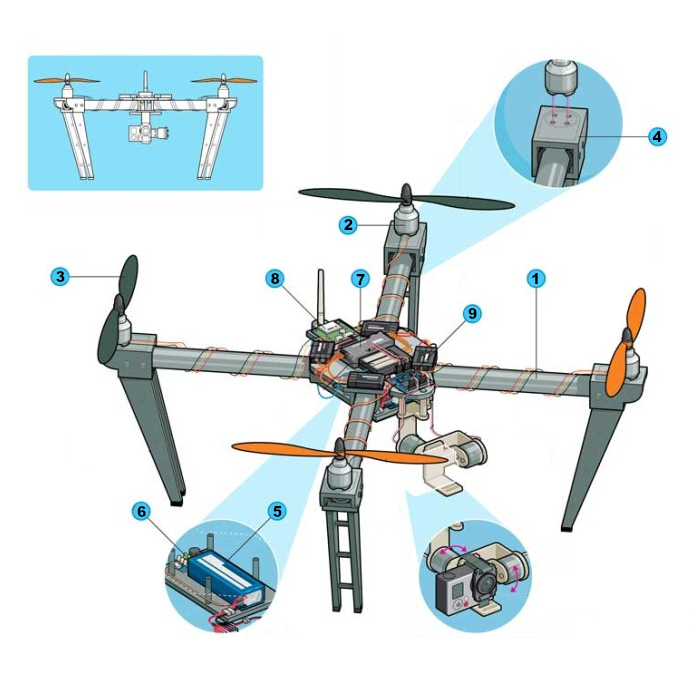
\includegraphics[width=0.5\textwidth]{soa/drone_hw_components}
    \caption[Drone hardware components]{The main hardware components of a drone are: 1. drone's frame, 2. motors, 3. propellers, 4. motor mount, 5. battery, 6. power distribution unit, 7. computing and memory unit, 8. communication unit, 9. sensors unit }
    \label{fig:drone_hw_components}
\end{SCfigure}

The software that runs on the drone, also known as the autopilot software, is usually composed of four main components: the communication unit, the sensing unit, the core control loop unit, and the low-level control unit. 
In Figure~\ref{fig:drone_sw_components}, we can see how the software components cooperate together to achieve a controllable and stable flight.
The communication unit receives and decodes commands from the off-board system; the signal is then transformed into power set-points from the core unit (control loop) with the help of sensor information. 
The sensing unit gathers information from the environment using sensors, translate 
sensor readings into readable values, then send this information to the core unit and to the communication unit to send back telemetry data to off-board systems.

\sidecaptionvpos{figure}{c}
\begin{SCfigure}[\sidecaptionrelwidth][tb]
    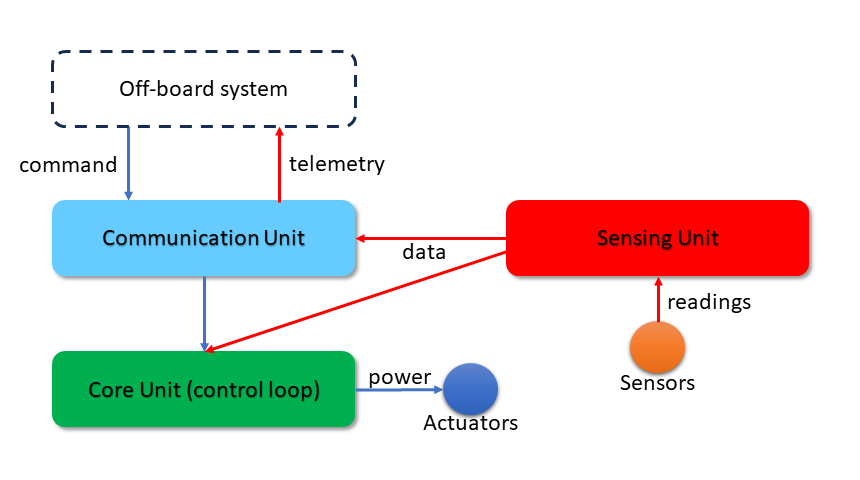
\includegraphics[width=0.7\textwidth]{soa/drone_sw_components.png}
    \caption[Drone software components]{
        The main software components of a drone are: 
        the \textit{sensing unit}, the \textit{communication unit} and the \textit{core unit (control loop)}.
    }\label{fig:drone_sw_components}
\end{SCfigure}

The current landscape of on-board drone solutions ranges from commercial off-the-shelf (COTS) to entirely custom solutions.
Commercial producers of drones like Parrot~\cite{parrot}, DJI~\cite{dij}, and 3DR~\cite{3DR} usually sell COTS solutions where all the hardware resources are supplied
with the software needed to run the drone.
Depending on the application, these bundled solutions may not be enough; if this is the case, 
the developer then needs to manually select each hardware component, control the compatibility with each other, 
and then select (or develop) the software that allows the drone to fly.

Some producer sell also intermediate solutions~\cite{pixhawk, px4, cube, navio2} between COTS and the completely custom one.
These solutions are composed of a microcontroller with usually the basic sensors that compose the 
Inertial Measurement Unit (IMU) and the autopilot software. 
These solutions are then extensible with other custom hardware; they provide programming tools to program the 
behavior of the drone during the flight.

%  TODO: reference chapter tools (section bitcraze) 
Regarding our setup, the on-board system that we used is a nano drone named Crazyflie 2.1, produced by Bitcraze; 
it is a COTS solution but with a lot of space for customization for both hardware and software components.

Off-board the drone, the environment is strongly related to the application scenario, and, in particular, it depends on the level of 
autonomy request for the drone, the flight area dimension, and the complexity of the operation.

Despite the heterogeneity of off-board systems, we can consistently identify two main components in most scenarios: a control unit and a communication unit. 
In most common situations, control and communication units are hosted on a single device.
Example of these devices are remote controls (Figure~\ref{fig:ground_station_controller}), smartphones (Figure~\ref{fig:ground_station_controller})
or a computer that acts as base (ground) station (Figure~\ref{fig:ground_base_station}).
When the scenario is more complex and the fight area is very broad, 
we can have a distributed ground network of control and communication units (Figure~\ref{fig:ground_station_distributed}).
Additionally, in combination with a distributed ground network, a sensor network can also be deployed to gather more information about the drone in its environment (Figure~\ref{fig:ground_station_distributed_with_sensor}). 
For example, the sensor network can be composed of sensors that collect atmospheric data, allowing for a better knowledge of the environment in which the drone is deployed. 

\begin{figure}[tb]
    \centering
    \subfloat[Remote control\label{fig:ground_station_controller}]{
        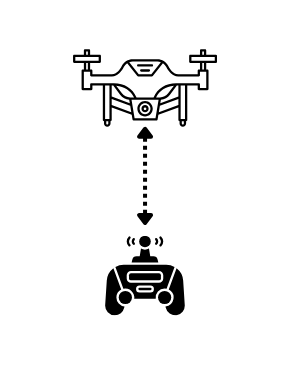
\includegraphics[width=0.25\textwidth]{soa/ground_station_controller}
    }
    \quad
    \subfloat[Smartphone\label{fig:ground_station_smartphone}]{
        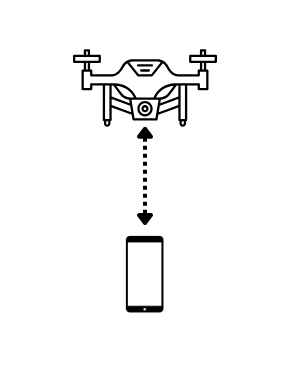
\includegraphics[width=0.25\textwidth]{soa/ground_station_smartphone}
    }
    \quad
    \subfloat[Base Station\label{fig:ground_base_station}]{
        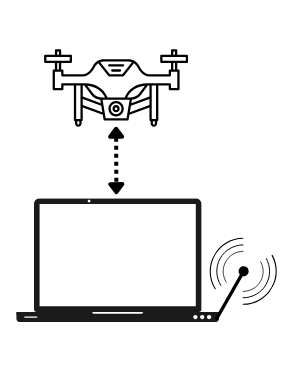
\includegraphics[width=0.25\textwidth]{soa/ground_base_station}
    }
    \quad
    \subfloat[Distributed ground network\label{fig:ground_station_distributed}]{
        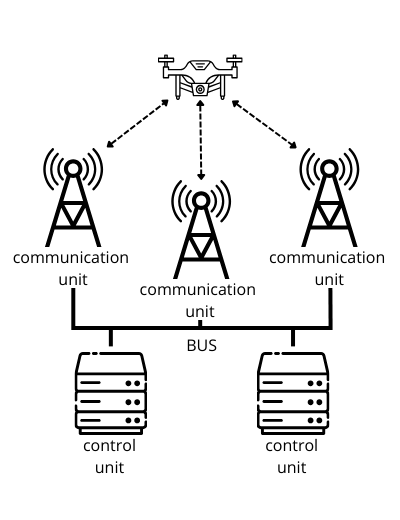
\includegraphics[width=0.35\textwidth]{soa/ground_station_distributed}
    }
    \quad
    \subfloat[Distributed ground network and sensor network\label{fig:ground_station_distributed_with_sensor}]{
        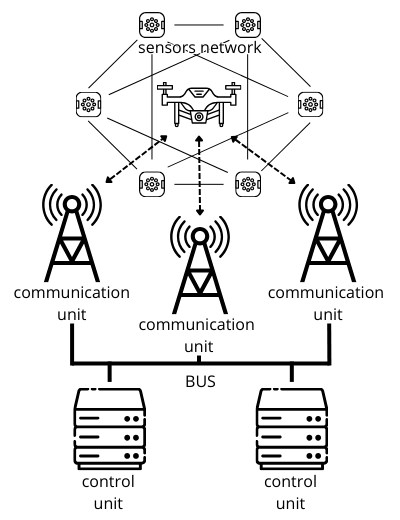
\includegraphics[width=0.35\textwidth]{soa/ground_station_distributed_with_sensor}
    }
    \caption[Off-board ecosystem]{Off-board ecosystem}\label{fig:off_board_ecosystem}
\end{figure}

Communication technology and infrastructure are critical topics that can introduce potential issues 
in the off-board environment when it is inadequate for the application scenario.
In particular, depending on the flight area's dimension, location, and topography, appropriate technology and communication infrastructure must be deployed to have a properly working drone.

As highlighted in Figure~\ref{fig:off_board_ecosystem}, the communication infrastructure can be single or distributed.
The former is more straightforward to implement and deploy but can be not enough when the flight area is too broad or the topography is irregular; 
the latter is much more complex but allows for covering all the possible application scenarios.

The most commonly used communication technology in the drone's field are Wi-Fi, radio, Bluetooth, and cellular network~\cite{pantelimon2019surveyCommunication}. 
Table~\ref{table:communication_technologies} summarizes the most common communication technologies and their characteristics.
Even if the research frontier for drone communication is mainly focused on cellular, in particular the 5G network~\cite{sharma2020communication},
none of the technologies prevails, but the choice depends on the application scenario. 
Cellular

can be a great solution around highly populated areas, while another technology must be considered in rural locations.


\begin{table}[tb]
    \centering
        \begin{tabular}{|c|c|c|c|c|}
        \hline
        \rowcolor{bluepoli!40}
        \textbf{Technology} & \textbf{Range} & \textbf{Weight} & \textbf{Complexity} & \textbf{Cost} \\
        \hline \hline
        Wi-Fi & MED [100m] & MED & HIGH & MED \\
        \hline
        Radio & SHORT-LONG [10-1000m] & LOW & LOW & LOW \\
        \hline
        Bluetooth & SHORT-MED [<25m] & LOW & MED & LOW \\
        \hline
        Cellular & LONG [8000m] & LOW & HIGH & MED \\
        \hline
        \end{tabular}
        \\[10pt]
        \caption[Communication technologies]{Communication technologies used in drone applications~\cite{pantelimon2019surveyCommunication}}\label{table:communication_technologies}
    \end{table}

The software that runs off-board is usually apt to coordinate all the resources of the environment to finally achieve and 
complete the task needed for the application. When using COTS or intermediate solutions, the vendors usually provide the 
hardware and software that compose the off-board ecosystem.

Figure~\ref{fig:easyfly_offboard_ecosystem} shows the off-board environment used in this work. 
It consists of a single base station with a USB dongle radio operating in a 2.4GHz band using a custom communication protocol named CRTP (see Section~\ref{subsec:crazyradio}). 
In substitution of a sensor network, we have an external positioning system (Lighthouse positioning system) composed of two base stations that beam the flight space with infrared, enabling the drone to measure its position by knowing the direction of infrared rays (see Section~\ref{subsec:lighthouse_hardware}).

\begin{wrapfigure}{H}{0.3\textwidth}
    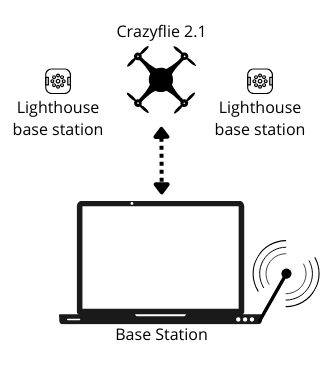
\includegraphics[width=0.3\textwidth]{soa/easyfly_offboard_ecosystem}
    \caption{EasyFly off-board ecosystem.}\label{fig:easyfly_offboard_ecosystem}
\end{wrapfigure}

A widespread problem encountered while dealing with drones is the testing phase of the application in a real environment. 
As in any other programming environment, drone programming is not immune to code bugs or hardware problems. 
Unfortunately, when an error arises, the drone will usually crash; in some unfortunate cases, some parts will break and need to be replaced. 
Therefore, testing drone applications is a very expensive task both in terms of economic resources and in terms of time. 

To overcome this limitation, the main drone producers have developed and distributed a simulation environment that allows 
testing the software before going into a real scenario. 
A simulation environment allows running the code written for the planned mission in a graphical simulation that shows the drone performing the tasks. 
Modern simulation environment~\cite{sphinx, DIJflightSimulator} usually takes into consideration atmospheric phenomena like pressure and wind to make the simulation 
closer to the real deployment environment.

In our work, we built our custom simulation tool, allowing us for a better evaluation of the work itself and, moreover, allowing  
users of our programming environment to have all the benefits of using a simulation environment (see Section~\ref{subsec:simulation_environment}).

\subsection{Swarm Programming}\label{subsec:swarm_programming}
In modern drone applications, where the tasks to achieve are complex, and the application has to be reliable, a common approach is 
to deploy multiple drones to complete the requested task collectively. This approach is completely different from single 
drone programming; in fact, swarm programming introduces new challenges and a different approach to achieving the tasks of the application.

Swarm programming is a branch of the more general swarm engineering which tries to take advantage of using multiple resources to 
achieve the application goal with better performance.

Swarm robotics and, more in general, swarm engineering is an emerging discipline that aims at defining systematic 
and well-founded procedures for modeling, designing, realizing, verifying, validating, operating, and maintaining 
a swarm robotics system. Taking inspiration from the self-organized behaviors of social animals, it makes use of simple 
rules and local interactions to design robust, scalable, and flexible collective behaviors for the coordination of large numbers of robots.
The inspiration that swarm robotics takes from the observation of social animals (ants, bees, birds, fish, …) is that starting from simple individuals,
they can become successful when they gather in groups, exhibiting a sort of swarm intelligence~\cite{bonabeau1999swarm}.

In particular, the behavior of social animal groups appears robust, scalable, and flexible. 
Robustness is the ability to cope with the loss of individuals. 
In social animals, robustness is promoted by redundancy and the absence of a leader. 
Scalability is the ability to perform well with different group sizes. 
The introduction or removal of individuals does not result in a drastic change in the performance of a swarm. 
In social animals, scalability is promoted by local sensing and communication. 
Flexibility is the ability to cope with a broad spectrum of different environments and tasks. 
In social animals, flexibility is promoted by redundancy, simplicity of the behaviors, and mechanisms such as task allocation.

Two great examples in the current literature of swarm engineering are Proto~\cite{bachrach2010proto} and Meld~\cite{ashley2007meld}. 
The former is a spatial computing language that allows programming swarms of robots starting from a mathematical model called amorphous medium.
The latter is a declarative programming language that uses logic programming to enable swarm programming.
Both languages directly take the swarm programming from the point of view of aggregate behaviors, i.e., their approach is to program the entire
swarm behavior instead of programming every single component separately.

When swarm robotics is applied in the field of drones, given the high dynamism in the movements of this type of robot, 
the swarm management and control is much more complex with respect to the single drone, 
but the capability of the swarm may increase the application's performance.

In the first place, the swarm, compared to the single drone, can provide a higher availability.
A single drone has a limited flight time, so its batteries need to be recharged or replaced. A swarm instead can dynamically 
deploy and retire drones to be always active on the field. In addition, a swarm can also scale when the request 
increases, e.g., a phenomenon to sense has a peak of occurrence~\cite{dantu2011karma}. 
In the same situation, a single drone application can miss the peak of the phenomena because, for example, it can be stuck at the charging station.

With swarms, the goal of the application is usually defined as a swarm goal.
Swarm goals are high-level goals whose achievement is independent of the success or the failure of the single task of a swarm component.
The separation between application (swarm) goals and drone tasks allows the application to be scalable and fault-tolerant.
Of course, the advantages of the swarm with respect to the single drone hide inside a huge complexity.
As the number of components of the swarm increases, the complexity of managing all of them increases, 
introducing a consistent overhead that can affect the application's performance.
As in any other engineering problem, we must select and identify the most suitable swarm size for the application to realize.

Depending on the application domain, we can adopt different strategies for coordinating the resources available.
We can identify three main programming models that can be applied to swarm programming in the field of drones: drone-level programming, swarm programming, and team-level programming.

Drone-level programming is the most straightforward approach; it expects to develop a single application for each component of the swarm, 
taking into account all the possible interactions between them. 
This finest grain method allows an entirely independent, customizable, and deterministic single-drone behavior. 
Since the application has a swarm goal that is not directly related to the single drone's task, 
with this method, it is usually tricky to use all the swarm resources efficiently to reach the general goal. 
Moreover, it has been proven~\cite{mottola2014team, dantu2011karma} that this method is indeed the most complex of the three in terms of programming effort.

Swarm programming~\cite{quigley2009ros}, on the other hand, allows writing a single set of rules that are common for all drones, and then every single drone 
executes that instruction in its local state. The swarm programming model explicitly forbids a shared or global state.
This programming model is easier to use and to set up and scale up with multiple drones, but it is challenging to represent tasks that require explicit drone coordination.

Team level programming~\cite{mottola2014team} is a programming model in between swarm and drone level programming, 
in which users express sophisticated collaborative sensing tasks without resorting to individual addressing 
and without exposure to the complexity of concurrent programming, parallel execution, scaling, and failure recovery.
The model can be viewed as a set of tasks that must be performed by a set of drones subject to particular timing and spatial constraints~\cite{mottola2014team}.

Our work does not address the complexity of swarm programming, although our programming environment, EasyFly, allows for the deployment of multiple drones (see Chapter~\ref{ch:conclusions}).


\chapter{Tools}
\label{ch:tools}
The main resource used in this work is Crazyflie, an open platform produced by Bitcraze~\cite{bitcraze} 
that offers an ecosystem of products and open-source libraries that allow people to develop new functionality for aerial drones. 

The key feature of this platform is that it offers a set of expansion decks that can extend the capabilities of the drone with new sensors. 
Expansion decks can be mounted on the drones very easily, and they are immediately ready to be used to compose the desired configuration in the application of interest.
Given its modularity and high versatility, this platform perfectly fits as a baseline for developing an easy, high-level environment for programming drones. 

The aim of this chapter is to present an overview of the Crazyflie platform to provide basic knowledge of its tools and surrounding environment.

% We will first present all the hardware used in this work, then we will give an overview of all the software libraries that compose the platform and finally we will describe in detail the main software components.

\section{Ecosystem Overview}\label{sec:ecosystem_oveerview}
The Crazyflie platform comprises a set of devices and tools to allow building drone applications. 
It has a modular architecture that makes it possible to build very versatile systems that are adaptable to many situations. 
In Figure~\ref{fig:bitcraze_ecosystem}, we can see an overview of the ecosystem of the entire platform.

The ecosystem of this platform gravitates around its leading actor: the Crazyflie 2.1 nano drone. 
In the basic settings, the drone has minimal sensors and actuators that allow it to fly. 
To empower the drone capabilities, the platform makes available a set of expansion decks that give the drone additional sensors, making it possible to adapt it to many possible situations.


\sidecaptionvpos{figure}{c}
\begin{SCfigure}[\sidecaptionrelwidth][h]
    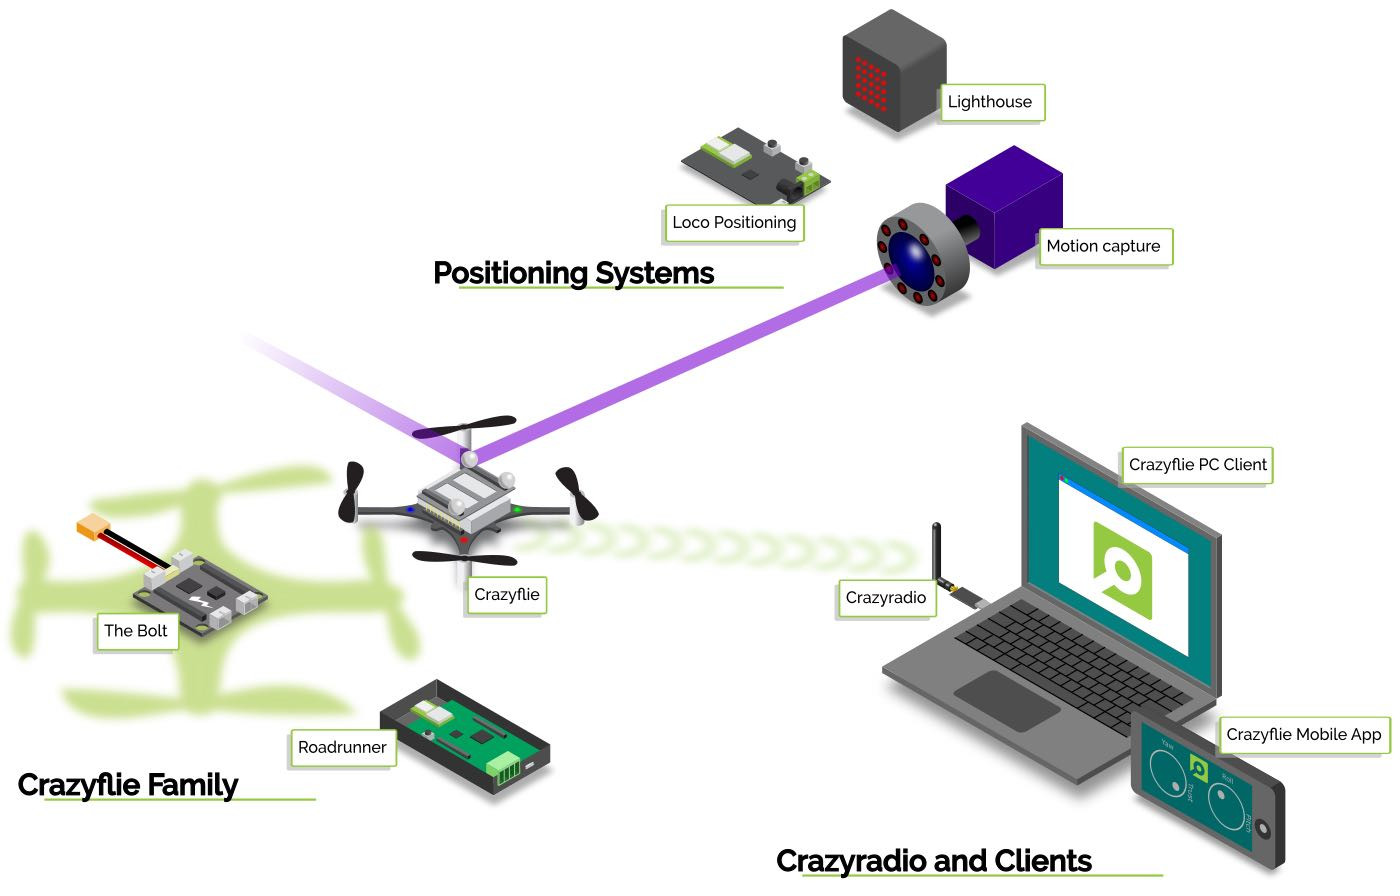
\includegraphics[width=0.5\textwidth]{tools/system_overview}
    \caption[Bitcraze Ecosystem overview]{This picture represents an overview of the Bitcraze Ecosystem~\cite{bitcraze}}
    \label{fig:bitcraze_ecosystem}
\end{SCfigure}


To coordinate the drone's operations, the platform needs a ground station that can be hosted on any computer 
with a Python script interpreter or a mobile phone with a dedicated App installed. 

The communication between the quadcopter and the ground station is handled using a dongle USB (CrazyRadio) or through Bluetooth when using the mobile App.

The platform also offers multiple absolute positioning systems that allow the drone to have better position estimation in an absolute coordinate system.

\section{Hardware}\label{sec:crazyflie_hardware}
In this section, we will provide an overview of the hardware components of the entire Crazyflie platform. 
We will first analyze the characteristics of the Crazyflie quadcopter used in this work, and then we will briefly introduce the relevant expansion decks. 
We will then give an overview of the hardware components that compose the absolute positioning system adopted for the work: the Lighthouse positioning system.

\subsection{The Quadcopter}\label{subsec:the_quadcopter}
Bitcraze produces a family of drones with similar hardware and firmware but different sizes and properties. 
The target for this work is the principal component of this family, the Crazyflie 2.1, a tiny and versatile quadcopter with a solid and modularized design that falls into the category of nano-drones.

As described in Section~\ref{sec:the_solution}, nano-drones are the most suitable typology for conducting investigations around HDI. 
The modular approach owned by Crazyflie 2.1 constitutes another key advantage in the field of human-drone interactions; 
the user can easily change the setup to address any possible situation. 

This drone has many hardware components hosted on a single, compact, light base. 
We can identify four main units: Computing Unit, Motor Unit, Sensor Unit, and Power Unit.

The core of the drone is composed of two Micro Controller Units (MCUs): 
The first is an STM32F4 MCU that handles the main Crazyflie firmware with all the low-level and high-level controls. 
The second MCU, NRF51822, handles all the radio communication and power management. 

The motor unit of the Crazyflie 2.1 consists of four Coreless DC motors with plastic propellers fixed at the corners of the base with the help of plastic supports.
To control the flight, the drone is equipped with two sensors: a BMI088 sensor, which measures the acceleration along the three coordinates of space plus the angular speed, 
and a BMP388 sensor, which is a high-precision pressure sensor.
The sensor unit of the Crazyflie 2.1, also known as the Inertial Measurement Unit (IMU), is minimal and provides the minimum data that allows the drone to have an almost stable flight.

Its design is robust and simple, easing the assembly and maintenance of its components.
Finally, the power unit is constituted by a 240mAh LiPo battery that allows a flight duration of about 7 minutes. 
The total weight of the drone is 27 grams, and it can lift a payload of 15 grams~\cite{crazyflie}. 


\subsection{Expansion Decks}\label{subsec:expansion_decks}
With only two sensors composing the IMU, the drone has a limited capacity to understand the surrounding environment. 
To overcome this limitation, the drone can be equipped with additional decks that extend its capabilities in sensing, positioning, and visualization.
The platform offers a variety of expansion decks, but for the purpose of our work, only a subset of them has been selected.
Figure~\ref{fig:decks} shows the expansion decks selected, particularly those that can enable in some way the human-drones interaction.

\begin{figure}[h]
    \centering
    \subfloat[Flow deck v2\label{fig:flow_deck}]{
        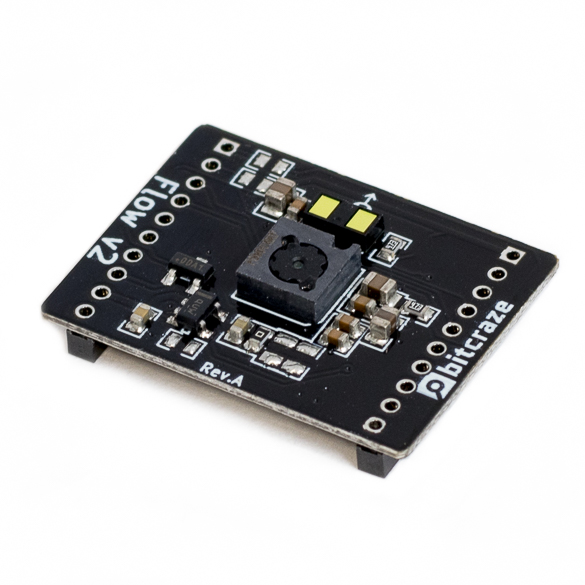
\includegraphics[width=0.16\textwidth]{tools/flow_deck_v2}
    }
    \quad
    \subfloat[Z-ranger deck v2\label{fig:z_ranger_deck}]{
        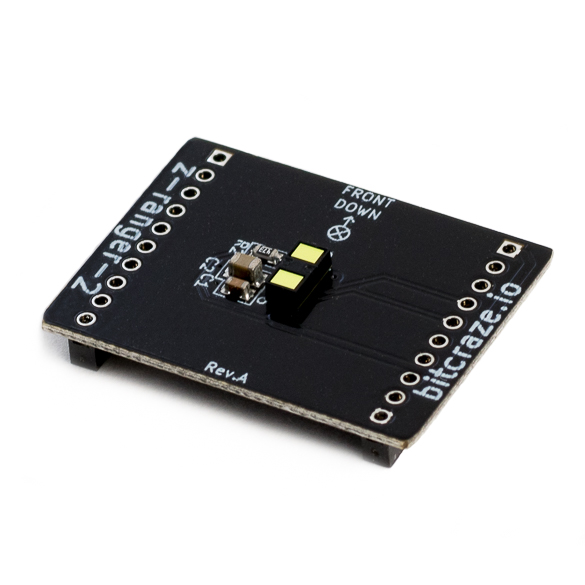
\includegraphics[width=0.16\textwidth]{tools/z-ranger_v2}
    }
    \quad
    \subfloat[Multi-ranger deck\label{fig:multi_ranger_deck}]{
        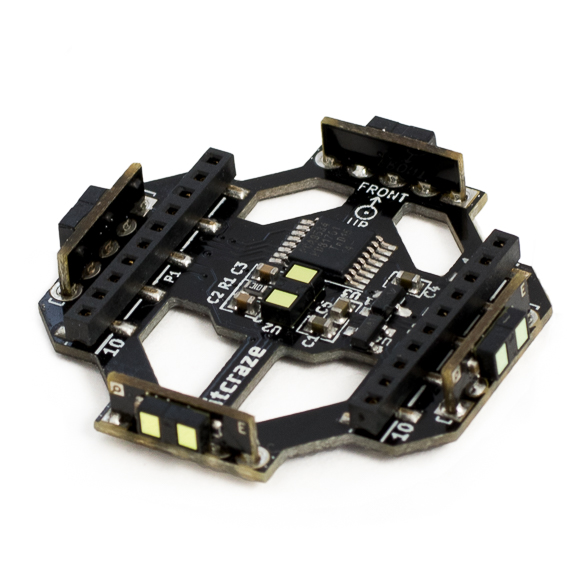
\includegraphics[width=0.16\textwidth]{tools/multi-ranger_deck}
    }
    \quad
    \subfloat[Lighthouse positioning deck\label{fig:lighthouse_deck}]{
        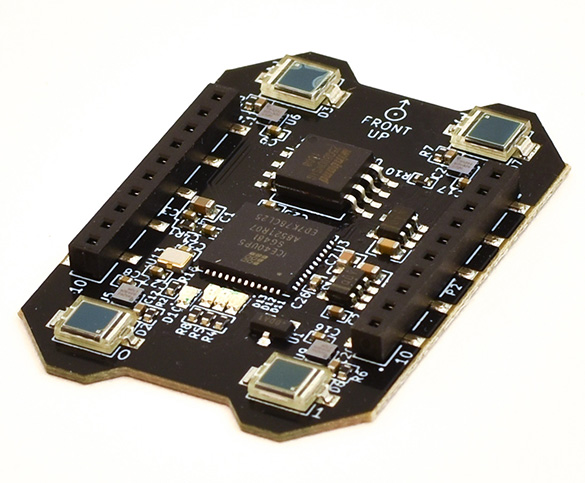
\includegraphics[width=0.16\textwidth]{tools/lighthouse_deck}
    }
    \quad
    \subfloat[AI-deck 1.1\label{fig:ai_deck}]{
        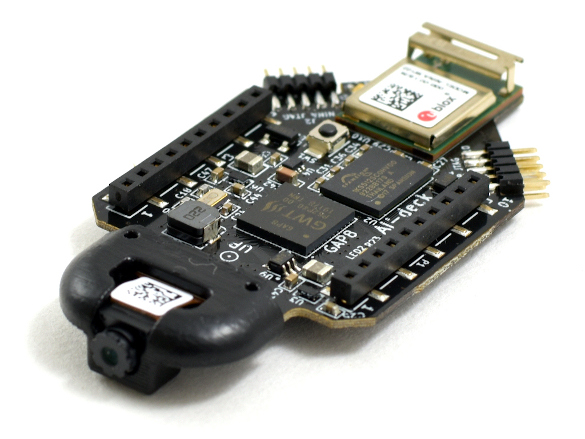
\includegraphics[width=0.16\textwidth]{tools/ai-deck}
    }
    \caption{Expansion decks of Crazyflie 2.1}\label{fig:decks}
\end{figure}


{\bfseries \scshape Flow deck v2}\label{deck:flow}:\\*
The Flow deck (Figure~\ref{fig:flow_deck}) allows the Crazyflie to understand when it moves in any direction. 
It mounts two sensors: the VL53L1x ToF measures the distance to the ground with high precision up to 4 meters, and the PMW3901 optical flow sensor measures the relative velocity in the x-y plane relative to the ground. 
This expansion deck is a relative positioning system that lets the drone know its position relative to its take-off point.

{\bfseries \scshape Z-ranger deck v2}\label{deck:z_ranger}:\\*
The Z-ranger deck (Figure~\ref{fig:z_ranger_deck}) is a simplified and cheaper version of the Flow deck v2.
It only measures the distance from the floor up to 4 meters using the usual laser sensor VL53L1x ToF.

{\bfseries \scshape Multi-ranger deck}\label{deck:multi_ranger}:\\*
The Multi-ranger deck (Figure~\ref{fig:multi_ranger_deck}) gives the Crazyflie the capability to sense the space around it and react when something is close and for instance, avoid obstacles.
This is done by measuring the distance to objects in the following five directions: front, back, left, right, and up with mm precision up to 4 meters, using five VL53L1x ToF sensors.


{\bfseries \scshape Lighthouse positioning deck}\label{deck:lighthouse}:\\*
The Lighthouse deck (Figure~\ref{fig:lighthouse_deck}) is part of the Lighthouse absolute positioning system (See Section~\ref{subsec:lighthouse_hardware}). 
It comprises four TS4231 IR receivers and an ICE40UP5K FPGA to process the signal received.
This expansion deck lets the drone know its position in an absolute coordinate system.

{\bfseries \scshape AI-deck 1.1}\label{deck:ai}:\\*
The AI-deck 1.1 (Figure~\ref{fig:ai_deck}) extends the computational capabilities and will enable complex artificial intelligence-based workloads to run onboard, with the possibility to achieve fully autonomous navigation capabilities. 
It mounts an Himax HM01B0 (ultra-low power \(320 \times 320\) monochrome camera), GAP8 (ultra-low power 8+1 core RISC-V MCU), NINA-W102 (ESP32 module for WiFi communication), and it has 512 Mbit HyperFlash and 64 Mbit HyperRAM memories. 


\subsection{Crazyradio PA}\label{subsec:crazyradio}
As previously described, the Crazyflie platform expects two nodes of computation: the ground station and the Crazyflie 2.1 itself. 
To communicate with the Crazyflie 2.1, which has an integrated radio, the ground station needs an external radio dongle. 
The platform provides a low-latency and long-range USB radio dongle, the Crazyradio PA.

The CrazyRadio PA is based on the nRF24LU1+ from Nordic Semiconductor, and it features a 20dBm power amplifier giving a range of up to 1km (line of sight).
The dongle comes pre-programmed with Crazyflie's compatible firmware.

The communication protocol used to communicate is the Crazy Radio Transfer Protocol (CRTP), 
which is a custom communication protocol of the Crazyflie platform. %(See section 3.7). TODO: understand if there is this section

\subsection{Lighthouse Positioning System Hardware}\label{subsec:lighthouse_hardware}
The Lighthouse positioning system is one of the possible solutions that Bitcraze offers to have an absolute positioning system for understanding the drone's coordinates inside the flight space. 
The hardware of this system is composed of 2 or more HTC-Vive/SteamVR Base Station 2.0. 
The role of these base stations is to lighten up the flight space with periodic infrared (IR) beams.

Onboard the Crazyflie 2.1, the Lighthouse expansion deck allows it to capture these IR beams thanks to four TS4231 IR receivers. 
The signal captured is then passed to an ICE40UP5K FPGA that computes the angle of incidence of the IR rays with signal processing. 
The position and the pose of the Craziflie are then finally computed from the main MCU of the Crazyflie 2.1 % (See section 3.4.x).TODO: understand if there is this section


\section{Software Libraries}\label{sec:software_libraries}
As previously anticipated, the Crazyflie environment is completed by a set of open-source libraries, 
publicly available on GitHub, which allow people to program all its components and devices, 
develop new features, or upgrade existing ones. Each library targets a specific system component and is completely independent of all the others. 
This section will briefly describe the two main libraries used as a baseline for our work. 

\subsection{crazyflie-lib-python}\label{subsec:crazyflie_lib_python}
The crazyflie-lib-python (cflib in short)~\cite{crazyflie-lib-python} is a software repository that consists of a Python library for programming scripts that control the behavior of the Crazyflie 2.1.
The library provides the base facilities to allow users to define the desired drone behavior in a Python script, abstracting from the low-level control mechanism.

As shown in Figure~\ref{fig:software_libraries}, the Python scripts are executed on the ground station.
The library contains the code to create communication packets sent through the Crazyradio reaching the Crazyflie, which will eventually execute the commands requested. 

\subsection{crazyflie-firmware}\label{subsec:crazyflie-firmware}
The crazyflie-firmware~\cite{crazyflie-firmware} is a software repository that contains all the firmware of Crazyflie 2.1. 
The firmware is written in C++ and handles the main autopilot on the STM32F4; it contains the driver of each possible expansion deck and controls all the communication on the opposite side of the cflib.


\begin{figure}[h]
    \centering
    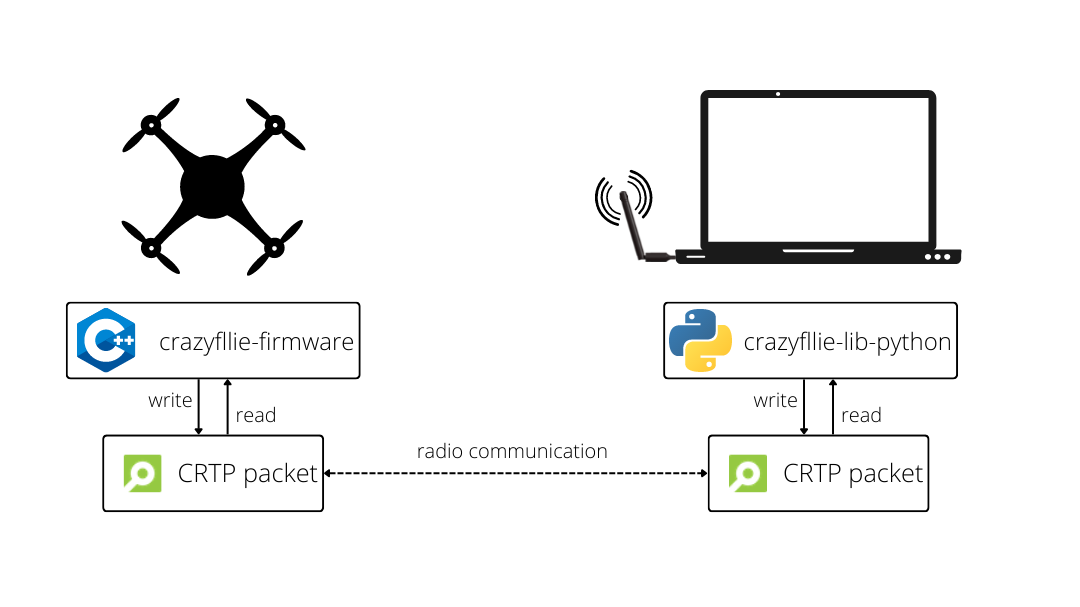
\includegraphics[width=0.9\textwidth]{tools/software_libraries}
    \caption[Software libraries integration]{
        The two main software libraries are \textit{crazyflie-firmware} and \textit{crazyflie-lib-python}. 
        The former, written in C++, runs on the drone; the latter, written in Python, runs on the base station. 
        The communication protocol that enables the cooperation of the two is the Crazy Radio Transfer Protocol (CRTP)}\label{fig:software_libraries}
\end{figure}


\section{Positioning Systems}\label{sec:positioning_systems}
Positioning systems represent the core sensing task of every drone application. 
Knowing the drone's position in the flight space is essential for achieving any possible goal.
We can identify two main categories of positioning systems: relative and absolute. 

Relative positioning systems are the simplest: starting from the drone's position at take-off, they estimate the position during the flight on the base of the movements made by the drone in the flight space. 
The measurement of the movements is usually made with the IMU (Inertial Measurement Unit) or with some additional sensors that track the difference in position over time.

The main issue related to this type of positioning system is that the error continually accumulates, and after a certain period of flight, they
can lead to consistent mispositioning.

Absolute positioning systems provide coordinates that define the exact location of an object within a specific coordinate system. 
These systems typically rely on external references or signals from fixed environmental points.
The sampling of the position in this type of positioning system is independent of any initial measurements, so the error in the positioning usually does not accumulate over time.


The Crazyflie platform offers multiple positioning systems, both absolute and relative. 
To select the best system for building our programming environment, we analyzed the following metrics for each possibility that the platform offered:
\begin{itemize}
    \item Relative or Absolute Positioning System
    \item Accuracy in sampling
    \item Cumulative of the error during time
\end{itemize}


\subsection{Relative Positioning Systems}\label{subsec:relative_positioning_systems}
The Crazyflie platform offers three relative positioning systems. 
The first system is represented by the Inertial Measurement Unit, which is provided on the base drone without expansion decks. 
From our experience, this system has very poor accuracy and cannot be used as the only positioning system of the entire application.
However, it contributes its information to obtain the position estimate.

The Z-ranger deck (See~\ref{deck:z_ranger}) is another positioning system that the platform offers; it provides an estimate only for the z-coordinate with pretty good accuracy, but, as typical for every relative positioning system, it has a high cumulative error during the time. 

The Flow deck v2 (See~\ref{deck:flow}) represents an empowered version of the Z-ranger, a positioning system capable of measuring the distance from the takeoff point for the three coordinates x, y, and z. 
This last system has a good sampling accuracy and an acceptable cumulative error rate over time. 
Flow deck v2 is the only relative positioning system that allows the Crazyflie to fly with acceptable precision in the flight space.


\subsection{Absolute Positioning Systems}\label{subsec:absolute_positioning_systems}
The environment provides three different absolute positioning systems solutions with different characteristics, performance, and costs. 

The first solution proposed, the Loco Positioning System (LPS), is based on Ultra Wide Band radio that is used to find the absolute 3D position of objects in space. 
Similarly to a miniature GPS system, it uses a set of Anchors, namely Loco positioning nodes (from 4 up to 8), that act as a GPS satellite, and a Tag, 
namely, the Loco positioning deck, which acts as a GPS receiver. 
As indicated in the specification of this system, the accuracy of this system is probably the main limitation and is estimated to be in the range of 10 cm. 

The second solution proposed is the Motion Capture System (MCS), which uses cameras to detect markers attached to the Crazyflies. 
Since the system knows the layout of the markers on the drone, it is possible to calculate the position and orientation of the tracked object in a global reference frame. 
It is a very accurate positioning system, but the two main limitations are that the native environment provides only the markers and relies on third-party systems for the entire MCS. 
Moreover, the position is computed in an external node and needs to be sent to the Crazyflie, increasing the communication load.

The last solution is the Lighthouse positioning system (Lighthouse), the newest introduced in the environment and selected for the work because it overcomes all the limitations of the previous.
Lighthouse is an optically-based positioning system that allows an object to locate itself with high precision indoors. 

The system uses the SteamVR Base Station (BS) as an optical beacon. 
They are composed of spinning drums that shine the flight space with infrared beams in a range of 6 meters. 

The Crazyflie, on the other hand, with a Lighthouse positioning deck with four optical IR receivers (photodiode), can measure the angle of incidence of the IR beams. 
Knowing the position and orientation of the BS enables the Crazyflie to compute its position onboard in global coordinates. 
The knowledge of the position and the orientation of the BS is called system geometry and is composed of a vector in the three dimensions and a rotation matrix. 



\section{State Estimate and Control}\label{sec:state_estimate_and_control}
All the information given by the positioning systems and by the additional decks are simply data,
to become useful, they need to be used cleverly to control the drone's stability and make it possible to fly. 

This section will describe the principal software components that act in the control loop, enabling the drone to fly.
In the Crazyflie platform, the control loop is managed inside the Crazyflie firmware (See~\ref{subsec:crazyflie-firmware}) from the sensor read to the motor thrust.
In Figure~\ref{fig:control_loop}, we can see a representation of the control loop of the Craziflie 2.1. 

\begin{figure}[h]
    \centering
    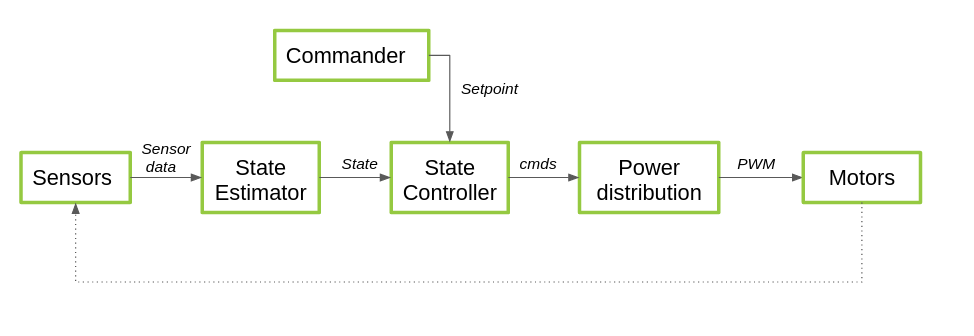
\includegraphics[width=0.9\textwidth]{tools/control_loop}
    \caption[Craziflie's control loop]{
        The control loop of the Craziflie 2.1~\cite{bitcraze}
    }\label{fig:control_loop}
\end{figure}

As in any feedback control system, also for the Crazyflie control loop, we can identify two principal components in Crazyflie 2.1: the state estimator and the state control. 
The synergy between the state estimate and the state control in a control loop is fundamental for achieving accurate and effective system control. 

The state estimator is responsible for computing the best possible estimate of the system's current status.
This component inside the Crazyflie 2.1 firmware has two concrete implementations with different performances and accuracy:
\begin{itemize}
    \item Complementary Filter
    \item Extended Kalman Filter (EKF)
\end{itemize}

The Complementary Filter is a very lightweight and efficient state estimator. 
It can only partially use the available sensors; in particular, it uses only data from the IMU and the ToF sensor (Flow deck or Z-ranger).
The estimated output is only a portion of the Crazyflie state: the Attitude (roll, pitch, and yaw) and the z coordinate relative to the starting point.

The EKF is a recursive filter that estimates the current state of the Crazyflie based on incoming measurements (in combination with a predicted standard deviation of the noise), the measurement model, and the model of the system itself. 
It is a step up in complexity with respect to the other estimator; it accepts all the possible sensors' data as input. 
If enough sensor data are available, it can compute a complete state estimation as output: Attitude, Position, and Velocity in all directions.
The choice of which state estimator to use can be forced by the user or automatically set. 
By default, the firmware uses the lighter Complementary Filter and switches to the EKF if more sensors are available.

The state control uses this estimate to elaborate the actions needed to change the current state to a target state.
On the Craziflie's 2.1 firmware, we have three possible alternatives, ordered by complexity:
\begin{itemize}
    \item Proportional Integral Derivative Controller (PID)
    \item Incremental Nonlinear Dynamic Inversion Controller (INDI)
    \item Mellinger controller
\end{itemize}


\section{Flight Control}\label{sec:flight_control}
On the other side of the communication channel, the ground station needs a way to interact with the drone and give information on which actions to take to fly in the desired way.

Inside the cflib the one responsible for controlling the flight is a module named Commander Framework.
The Commander Framework can be viewed as composed of two layers:

The first layer provides low-level operations that allow writing setpoints and sending them with the custom CRTP protocol.

The second layer, built upon the first, is more abstract and adds some general functionalities, e.g., take-off, land, and move-to.



\chapter{Chapter one}
\label{ch:chapter_one}%
% The \label{...}% enables to remove the small indentation that is generated, always leave the % symbol.

In this chapter additional useful information are reported.

\section{Sections and subsections}
\label{sec:section_name}
Chapters are typically subdivided into sections and subsections, and, optionally,
subsubsections, paragraphs and subparagraphs.
All can have a title, but only sections and subsections are numbered.
A new section is created by the command
\begin{verbatim}
\section{Title of the section}
\end{verbatim}
The numbering can be turned off by using \verb|\section*{}|.
\\
A new subsection is created by the command
\begin{verbatim}
\subsection{Title of the subsection}
\end{verbatim}
and, similarly, the numbering can be turned off by adding an asterisk as follows 
\begin{verbatim}
\subsection*{}
\end{verbatim}

\section{Equations}
\label{sec:eqs}
This section gives some examples of writing mathematical equations in your thesis.

Maxwell's equations read:
\begin{subequations}
    \label{eq:maxwell}
    \begin{align}[left=\empheqlbrace]
    \nabla\cdot \bm{D} & = \rho, \label{eq:maxwell1} \\
    \nabla \times \bm{E} +  \frac{\partial \bm{B}}{\partial t} & = \bm{0}, \label{eq:maxwell2} \\
    \nabla\cdot \bm{B} & = 0, \label{eq:maxwell3} \\
    \nabla \times \bm{H} - \frac{\partial \bm{D}}{\partial t} &= \bm{J}. \label{eq:maxwell4}
    \end{align}
\end{subequations}

Equation~\eqref{eq:maxwell} is automatically labeled by \texttt{cleveref},
as well as Equation~\eqref{eq:maxwell1} and Equation~\eqref{eq:maxwell3}.
Thanks to the \verb|cleveref| package, there is no need to use \verb|\eqref|.
Remember that Equations have to be numbered only if they are referenced in the text.

Equations~\eqref{eq:maxwell_multilabels1}, \eqref{eq:maxwell_multilabels2}, \eqref{eq:maxwell_multilabels3}, and \eqref{eq:maxwell_multilabels4} show again Maxwell's equations without brace:
\begin{align}
    \nabla\cdot \bm{D} & = \rho, \label{eq:maxwell_multilabels1} \\
    \nabla \times \bm{E} +  \frac{\partial \bm{B}}{\partial t} &= \bm{0}, \label{eq:maxwell_multilabels2} \\
    \nabla\cdot \bm{B} & = 0, \label{eq:maxwell_multilabels3} \\
    \nabla \times \bm{H} - \frac{\partial \bm{D}}{\partial t} &= \bm{J} \label{eq:maxwell_multilabels4}.
\end{align}

Equation~\eqref{eq:maxwell_singlelabel} is the same as before,
but with just one label:
\begin{equation}
    \label{eq:maxwell_singlelabel}
    \left\{
    \begin{aligned}
    \nabla\cdot \bm{D} & = \rho, \\
    \nabla \times \bm{E} +  \frac{\partial \bm{B}}{\partial t} &= \bm{0},\\
    \nabla\cdot \bm{B} & = 0, \\
    \nabla \times \bm{H} - \frac{\partial \bm{D}}{\partial t} &= \bm{J}.
    \end{aligned}
    \right.
\end{equation}

\section{Figures, Tables and Algorithms}
Figures, Tables and Algorithms have to contain a Caption that describe their content, and have to be properly reffered in the text.

\subsection{Figures}
\label{subsec:figures}

For including pictures in your text you can use \texttt{TikZ} for high-quality hand-made figures,
or just include them as usual with the command
\begin{verbatim}
\includegraphics[options]{filename.xxx}
\end{verbatim}
Here xxx is the correct format, e.g. \verb|.png|, \verb|.jpg|, \verb|.eps|, \dots.

\begin{figure}[H]
    \centering
    
\includegraphics[width=0.3\textwidth]{logo_polimi_scritta.eps}
    \caption{Caption of the Figure to appear in the List of Figures.}
    \label{fig:quadtree}
\end{figure}

Thanks to the \texttt{\textbackslash subfloat} command, a single figure, such as Figure~\ref{fig:quadtree},
can contain multiple sub-figures with their own caption and label, e.g. \color{black} Figure~\ref{fig:polimi_logo1} and Figure~\ref{fig:polimi_logo2}. 

\begin{figure}[H]
    \centering
    \subfloat[One PoliMi logo.\label{fig:polimi_logo1}]{
        
\includegraphics[scale=0.5]{Images/logo_polimi_scritta.eps}
    }
    \quad
    \subfloat[Another one PoliMi logo.\label{fig:polimi_logo2}]{
        
\includegraphics[scale=0.5]{Images/logo_polimi_scritta2.eps}
    }
    \caption[Shorter caption]{This is a very long caption you don't want to appear in the List of Figures.}
    \label{fig:quadtree2}
\end{figure}


\subsection{Tables}
\label{subsec:tables}

Within the environments \texttt{table} and  \texttt{tabular} you can create very fancy tables as the one shown in Table~\ref{table:example}.
\begin{table}[H]
    \caption*{\textbf{Title of Table (optional)}}
    \centering 
    \begin{tabular}{|p{3em} c c c |}
    \hline
    \rowcolor{bluepoli!40} % comment this line to remove the color
     & \textbf{column 1} & \textbf{column 2} & \textbf{column 3} \T\B \\
    \hline \hline
    \textbf{row 1} & 1 & 2 & 3 \T\B \\
    \textbf{row 2} & $\alpha$ & $\beta$ & $\gamma$ \T\B\\
    \textbf{row 3} & alpha & beta & gamma \B\\
    \hline
    \end{tabular}
    \\[10pt]
    \caption{Caption of the Table to appear in the List of Tables.}
    \label{table:example}
\end{table}

You can also consider to highlight selected columns or rows in order to make tables more readable.
Moreover, with the use of \texttt{table*} and the option \texttt{bp} it is possible to align them at the bottom of the page. One example is presented in Table~\ref{table:exampleC}. 

\begin{table}[H]
\centering 
    \begin{tabular}{|p{3em} | c | c | c | c | c | c|}
    \hline
%    \rowcolor{bluepoli!40}
     & \textbf{column1} & \textbf{column2} & \textbf{column3} & \textbf{column4} & \textbf{column5} & \textbf{column6} \T\B \\
    \hline \hline
    \textbf{row1} & 1 & 2 & 3 & 4 & 5 & 6 \T\B\\
    \textbf{row2} & a & b & c & d & e & f \T\B\\
    \textbf{row3} & $\alpha$ & $\beta$ & $\gamma$ & $\delta$ & $\phi$ & $\omega$ \T\B\\
    \textbf{row4} & alpha & beta & gamma & delta & phi & omega \B\\
    \hline
    \end{tabular}
    \\[10pt]
    \caption{Highlighting the columns}
    \label{table:exampleC}
\end{table}

\begin{table}[H]
\centering 
    \begin{tabular}{|p{3em} c c c c c c|}
    \hline
%    \rowcolor{bluepoli!40}
     & \textbf{column1} & \textbf{column2} & \textbf{column3} & \textbf{column4} & \textbf{column5} & \textbf{column6} \T\B \\
    \hline \hline
    \textbf{row1} & 1 & 2 & 3 & 4 & 5 & 6 \T\B\\
    \hline
    \textbf{row2} & a & b & c & d & e & f \T\B\\
    \hline
    \textbf{row3} & $\alpha$ & $\beta$ & $\gamma$ & $\delta$ & $\phi$ & $\omega$ \T\B\\
    \hline
    \textbf{row4} & alpha & beta & gamma & delta & phi & omega \B\\
    \hline
    \end{tabular}
    \\[10pt]
    \caption{Highlighting the rows}
    \label{table:exampleR}
\end{table}

\subsection{Algorithms}
\label{subsec:algorithms}

Pseudo-algorithms can be written in \LaTeX{} with the \texttt{algorithm} and \texttt{algorithmic} packages.
An example is shown in Algorithm~\ref{alg:var}.
\begin{algorithm}[H]
    \label{alg:example}
    \caption{Name of the Algorithm}
    \label{alg:var}
    \label{protocol1}
    \begin{algorithmic}[1]
    \STATE Initial instructions
    \FOR{$for-condition$}
    \STATE{Some instructions}
    \IF{$if-condition$}
    \STATE{Some other instructions}
    \ENDIF
    \ENDFOR
    \WHILE{$while-condition$}
    \STATE{Some further instructions}
    \ENDWHILE
    \STATE Final instructions
    \end{algorithmic}
\end{algorithm} 

\vspace{5mm}

\section{Theorems, propositions and lists}

\subsection{Theorems}
Theorems have to be formatted as:
\begin{theorem}
\label{a_theorem}
Write here your theorem. 
\end{theorem}
\textit{Proof.} If useful you can report here the proof.

\subsection{Propositions}
Propositions have to be formatted as:
\begin{proposition}
Write here your proposition.
\end{proposition}

\subsection{Lists}
How to  insert itemized lists:
\begin{itemize}
    \item first item;
    \item second item.
\end{itemize}
How to insert numbered lists:
\begin{enumerate}
    \item first item;
    \item second item.
\end{enumerate}

\section{Use of copyrighted material}

Each student is responsible for obtaining copyright permissions, if necessary, to include published material in the thesis.
This applies typically to third-party material published by someone else.

\section{Plagiarism}

You have to be sure to respect the rules on Copyright and avoid an involuntary plagiarism.
It is allowed to take other persons' ideas only if the author and his original work are clearly mentioned.
As stated in the Code of Ethics and Conduct, Politecnico di Milano \textit{promotes the integrity of research,
condemns manipulation and the infringement of intellectual property}, and gives opportunity to all those
who carry out research activities to have an adequate training on ethical conduct and integrity while doing research.
To be sure to respect the copyright rules, read the guides on Copyright legislation and citation styles available
at:
\begin{verbatim}
https://www.biblio.polimi.it/en/tools/courses-and-tutorials
\end{verbatim}
You can also attend the courses which are periodically organized on "Bibliographic citations and bibliography management".

\section{Bibliography and citations}
Your thesis must contain a suitable Bibliography which lists all the sources consulted on developing the work.
The list of references is placed at the end of the manuscript after the chapter containing the conclusions.
We suggest to use the BibTeX package and save the bibliographic references  in the file \verb|Thesis_bibliography.bib|.
This is indeed a database containing all the information about the references. To cite in your manuscript, use the \verb|\cite{}| command as follows:
\\
\textit{Here is how you cite bibliography entries: \cite{knuth74}, or multiple ones at once: \cite{knuth92,lamport94}}.
\\
The bibliography and list of references are generated automatically by running BibTeX \cite{bibtex}.

\chapter{Conclusions and future developments}
\label{ch:conclusions}%
A final chapter containing the main conclusions of your research/study
and possible future developments of your work have to be inserted in this chapter.

%-------------------------------------------------------------------------
%	BIBLIOGRAPHY
%-------------------------------------------------------------------------

\addtocontents{toc}{\vspace{2em}} % Add a gap in the Contents, for aesthetics
\bibliography{Thesis_bibliography} % The references information are stored in the file named "Thesis_bibliography.bib"

%-------------------------------------------------------------------------
%	APPENDICES
%-------------------------------------------------------------------------

\cleardoublepage
\addtocontents{toc}{\vspace{2em}} % Add a gap in the Contents, for aesthetics
\appendix
\chapter{Appendix A}
If you need to include an appendix to support the research in your thesis, you can place it at the end of the manuscript.
An appendix contains supplementary material (figures, tables, data, codes, mathematical proofs, surveys, \dots)
which supplement the main results contained in the previous chapters.

\chapter{Appendix B}
It may be necessary to include another appendix to better organize the presentation of supplementary material.


% LIST OF FIGURES
\listoffigures

% LIST OF TABLES
\listoftables

% LIST OF SYMBOLS
% Write out the List of Symbols in this page
\chapter*{List of Symbols} % You have to include a chapter for your list of symbols (
\begin{table}[H]
    \centering
    \begin{tabular}{lll}
        \textbf{Variable} & \textbf{Description} & \textbf{SI unit} \\\hline\\[-9px]
        $\bm{u}$ & solid displacement & m \\[2px]
        $\bm{u}_f$ & fluid displacement & m \\[2px]
    \end{tabular}
\end{table}

% ACKNOWLEDGEMENTS
\chapter*{Acknowledgements}
Here you might want to acknowledge someone.

\cleardoublepage

\end{document}
